%\part{Temporal networks}
\chapter{Temporal network analysis}
The previous chapter has demonstrated that network analysis provides a deep insight into the processes behind epidemic spreading.
Given a sufficient amount of data, a contact network is capable to capture all possible infection pathways in the system.
The potential of static network analysis lies in the huge toolbox of methods that has been developed in the last decades.
As depicted in section \ref{sec:network_theory}, there exist coherent definitions for both their large scale topological features and local centrality measures allowing for node rankings.

Nevertheless, the concept of static networks neglects temporal variations in the system, i.e. the edges of a particular network are not necessarily present all the time.
This chapter addresses some of the conceptional problems owing to a sparse and heterogenous occurrence of edges in the network, the most central one being the \emph{causality of paths} in the network.
Section \ref{sec:Plos} focusses on the computational analysis of the full temporal representation of the network analyzed (from the static perspective) in section \ref{sec:network_analysis}.
In section \ref{sec:PRL}, we present a novel formalism mapping the causality of temporal networks onto a mathematical graph.

\section{Introduction}
To begin with, we highlight the most fundamental difference between static and temporal networks.
In particular, we compare the static and the temporal representation of the system.
Figure \ref{fig:temporal_network_principle} shows a temporal network and its aggregated graph.
%
\begin{figure}[htb]
\begin{center}
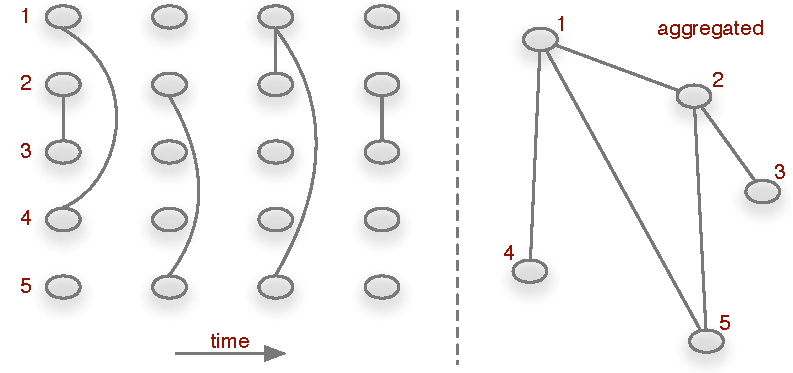
\includegraphics{Temporal_Network_Principle.pdf}
\caption{%
Role of causality in a temporal network with $5$ nodes and $T=4$.
The left panel shows snapshots of the system at different times and the right panel shows the corresponding aggregated network.
Although there is a path from node $3$ to $4$ (and vice versa) in the aggregated network (right panel), there is no causal path between $3$ and $4$ in the temporal network (left panel).
}
\label{fig:temporal_network_principle}
\end{center}
\end{figure}
%
Although the edges of the temporal network are present in the aggregated graph, the situation becomes more complex, if we consider paths of length greater than one.
The aggregated graph (right panel in figure \ref{fig:temporal_network_principle}) suggests that the network is connected, i.e. there is a path between every node pair.
As an example, there are two different paths from node $3$ to $4$ in the aggregated system.
However, this does not hold for the temporal system.
Consequently, paths in an aggregated graph of a temporal network have to be treated with care.

Before we give a formal definition of temporal networks, we have to distinguish between terms used for temporal networks and other systems.

\paragraph{Disambiguation\color{Cayenne}{.}}
Since the analysis of temporal networks is an interdisciplinary field, there is still no consistent designation for what the author refers to as \emph{temporal networks} \citep{Holme_review}.
Different phrases, such as temporal graphs, dynamic graphs, dynamic networks are used in the literature.
In addition to that, there are other classes of networks seeming to be related to temporal networks, i.e. adaptive networks, growing networks, evolving graphs.
The analysis of the latter has a strong focus on network growth, i.e. the process behind the evolution of static networks.
A central question for these systems is what is the fundamental process that has formed the network.
An example is the \BA network, where the underlying process is a rich-get-richer principle that results in a scale free degree distribution.
The striking difference between growing networks and temporal networks is that the snapshots of a temporal network can in principle be arbitrary.
Correlations between two snapshots of the system (if any) could be over arbitrary periods of time.
We prefer the term temporal network, since \emph{temporal} is not so easily confused with dynamic systems.
Furthermore, the systems under consideration are not mathematical graphs; therefore, we use the more general term \emph{network}.

\paragraph{Formal definition\color{Cayenne}{.}}
A temporal network $\mathcal{G}=(V,\mathcal{E},T)$ consists of a set of nodes $V$ and a set of edges $\mathcal{E}$, where each edge in $\mathcal{E}$ is given by a triple $(u,v,t)$ and connects nodes $u$ and $v$ at time $t\in T$.
$T$ is the observation period of $\mathcal{G}$, where $T\subset \mathbb{N}^+$ for time discrete systems and $T\subset \mathbb{R}^+$ for continuous systems.
\footnote{
In this work, we focus on time discrete systems, since a continuous time process can be approximated by a discrete one by choosing an appropriately small increment.
Furthermore, edge weights and a latency functions for edge traversal could be added to the definition \citep{Casteights_review}.
This is, however, beyond the scope of this thesis.
}
The aggregated graph $G=(V,E)$ of a temporal network simply ignores the occurrence times of the edges in $\mathcal{E}$ and the set of nodes $V$ is the same in both representations.


\paragraph{Viewpoints and implementation\color{Cayenne}{.}}
As in the case of static networks, temporal networks can be implemented in different ways.
A brief report of different implementations of static networks is given in Appendix \ref{sec:implementation}.
Besides the adjacency matrix, edge lists and adjacency lists are appropriate network representations.
Considering a temporal network as a sequence of static networks (called snapshots or graphlets) can be seen as a \emph{graph centric} view on the system.
It is the analogue of the adjacency matrix in static networks.
More formally, a temporal network $\mathcal{G}$ is represented by a sequence of adjacency matrices
\begin{equation}\label{eq:AdMatrixSequence}
\mathcal{A}=\mat{A}_1,\dots ,\mat{A}_T,
\end{equation}
where $T$ is the observation time and the increment is the temporal resolution.

In analogy to the edge lists of static networks (see Appendix \ref{sec:implementation}), an \emph{edge centric} view on a temporal network consists of the occurrence times of the edges.
Let $\mathcal{G}=(V,\mathcal{E})$ be a temporal network.
Than the set of edges $\mathcal{E}$ is represented by a sequence of triples
\begin{equation*}%\label{eq:temporal_edges}
\mathcal{E}=(u_1,v_1,t_1),(u_1,v_1,t_2),(u_2,v_2,t_2),\dots \;.
\end{equation*}
An edge centric view focusses on the occurrence times of each edge, i.e.
\[
\mathcal{I}((u_1,v_1))=t_2,t_2,\dots \; .
\]
This point of view is particularly convenient for the time randomization of temporal networks (see section \ref{sec:randomized_models_tvg}).
Finally, a \emph{node centric} view of a temporal network considers the neighborhood $\mathcal{N}$ of a node $v$ over time, i.e. $\mathcal{N}(v,t)$.
This view corresponds to the adjacency list of a static network (see Appendix \ref{sec:implementation}).
The temporal degree of each node immediately follows from $d(v,t)=\abs{\mathcal{N}(v,t)}$.

We focus on the \emph{graph centric view} \eqref{eq:AdMatrixSequence} of temporal networks in the rest of this thesis and make use of edge and node centric views implicitly in computer implementations.





\section{Data driven network analysis}\label{sec:Plos}
In order to be congruent with the datasets used in the publications, we use the pig trade dataset of \citep{Konschake:2013js} in this chapter.
This dataset differs slightly from the dataset in section \ref{sec:network_analysis}.
It covers the period from 01 January 2008 to 31 December 2009.
The results do not change qualitatively and results of \citep{Konschake:2013js} and \citep{Lentz:2013PRL} are comparable.


\subsection{Representative sample}

\subsection{Node rankings}

\paragraph{Correlations vs. Intersections\color{Cayenne}{.}}

\subsection{Temporal vs. static representation}

\section{Formalism driven network analysis}\label{sec:PRL}

\subsection{Matrices for temporal networks}

\subsection{Representative sample / characteristic time scale}

\subsection{Causal fidelity}

\subsection{Temporal and topological mixing patterns}

\subsection{Randomized models}\label{sec:randomized_models_tvg}







